\documentclass[landscape,final,a0paper]{baposter}

\usepackage{graphicx}
\usepackage[font=small,labelfont=bf]{caption}
\usepackage{amsmath, amssymb}
\usepackage{relsize, multirow, multicol}
\usepackage{times, helvet, palatino}
\usepackage{pgfbaselayers}

\pgfdeclarelayer{background}
\pgfdeclarelayer{foreground}
\pgfsetlayers{background,main,foreground}

\selectcolormodel{cmyk}
\setlength{\columnsep}{0.7em}
\setlength{\columnseprule}{0mm}

\newcommand{\compresslist}{
    \setlength{\itemsep}{1pt}
    \setlength{\parskip}{0pt}
    \setlength{\parsep}{0pt}}

\newcommand{\colouredcircle}[1]{%
      \tikz{\useasboundingbox (-0.2em,-0.32em) rectangle(0.2em,0.32em); \draw[draw=black,fill=baposterBGone!80!black!#1!white,line width=0.03em] (0,0) circle(0.18em);}}

\newcommand{\st}{\mathrm{st}}

\newcommand{\triangliff}{\mathrel{\overset\triangle\iff}}

\newcommand{\Los}{{\L}o\'s}

\begin{document}

% Define some colors
\definecolor{silver}{cmyk}{0,0,0,0.3}
\definecolor{yellow}{cmyk}{0,0,0.9,0.0}
\definecolor{reddishyellow}{cmyk}{0,0.22,1.0,0.0}
\definecolor{black}{cmyk}{0,0,0.0,1.0}
\definecolor{darkYellow}{cmyk}{0,0,1.0,0.5}
\definecolor{darkSilver}{cmyk}{0,0,0,0.1}
\definecolor{lightyellow}{cmyk}{0,0,0.3,0.0}
\definecolor{lighteryellow}{cmyk}{0,0,0.1,0.0}
\definecolor{lighteryellow}{cmyk}{0,0,0.1,0.0}
\definecolor{lightestyellow}{cmyk}{0,0,0.05,0.0}
\definecolor{cyan}{cmyk}{1,0,0,0}
\definecolor{lightcyan}{cmyk}{0.5,0,0,0}
\definecolor{pastelcyan}{cmyk}{0.25,0,0,0}
\definecolor{magenta}{cmyk}{0,1,0,0}
\definecolor{yellow}{cmyk}{0,0,1,0}
\definecolor{lightyellow}{cmyk}{0,0,0.5,0}
\definecolor{pastelyellow}{cmyk}{0,0,0.25,0}
\definecolor{black}{cmyk}{0,0,0,1}
\definecolor{darkgray}{cmyk}{0,0,0,0.75}
\definecolor{gray}{cmyk}{0,0,0,0.5}
\definecolor{lightgray}{cmyk}{0,0,0,0.25}
\definecolor{white}{cmyk}{0,0,0,0}
\definecolor{red}{cmyk}{0,1,1,0}
\definecolor{orange}{cmyk}{0,0.5,1,0}
\definecolor{scarlet}{cmyk}{0,1,0.5,0}
\definecolor{brown}{cmyk}{0.5,0.75,1,0}
\definecolor{camel}{cmyk}{0.25,0.375,0.5,0}
\definecolor{cream}{cmyk}{0,0.2,0.3,0}
\definecolor{green}{cmyk}{1,0,1,0}
\definecolor{lightgreen}{cmyk}{0.5,0,0.5,0}
\definecolor{pastelgreen}{cmyk}{0.25,0,0.25,0}
\definecolor{mossgreen}{cmyk}{0.64,0.4,1,0}
\definecolor{yellowgreen}{cmyk}{0.5,0,1,0}
\definecolor{skyblue}{cmyk}{0.4,0.16,0,0}
\definecolor{royal}{cmyk}{1.0,0.5,0,0}
\definecolor{navyblue}{cmyk}{0.9,0.75,0.5,0}
\definecolor{lightnavy}{cmyk}{0.4,0.3,0.2,0}
\definecolor{blue}{cmyk}{1,1,0,0}
\definecolor{lightblue}{cmyk}{0.5,0.5,0,0}
\definecolor{pastelblue}{cmyk}{0.25,0.25,0,0}
\definecolor{lightpastelblue}{cmyk}{0.15,0.15,0,0}
\definecolor{lightestpastelblue}{cmyk}{0.05,0.05,0,0}
\definecolor{lavender}{cmyk}{0.25,0.25,0,0}
\definecolor{violet}{cmyk}{0.75,1,0.25,0}
\definecolor{purple}{cmyk}{0.5,1,0.5,0}
\definecolor{lightpurple}{cmyk}{0.25,0.5,0.25,0}
\definecolor{pink}{cmyk}{0,0.5,0,0}


%%

\typeout{Poster Starts}
%\background{
  %\begin{tikzpicture}[remember picture,overlay]%
  %  \draw (current page.north west)+(-2em,-2em) node[anchor=north west] %{\hspace{-2em}\includegraphics[height=1.1\textheight]{silhouettes_background}};
 % \end{tikzpicture}%
%}




\newlength{\leftimgwidth}
\begin{poster}
  { colspacing=0.5em,
    bgColorOne=white, bgColorTwo=white,
    borderColor=navyblue,
    headerColorOne=navyblue,
    headerFontColor=white,
    boxColorOne=white,
    textborder=roundedleft,
    headerborder=open,
    headershape=roundedright,
    headerheight=0.08\textheight,
    headershade=plain,
    headerfont=\Large\textsf}
  {}
  {\vspace{-0.5em} \sf Ultraproducts and hyperreal analysis}
  {\sf \vspace{1.2em} 
  Abhimanyu Pallavi Sudhir }
  { \makebox[8em][r]{%
        \begin{minipage}{16em}
        \hfill \includegraphics[height=3em]{imperial.pdf}
        \end{minipage} } }

  \tikzstyle{light shaded}=[top color=baposterBGtwo!30!white,bottom color=baposterBGone!30!white,shading=axis,shading angle=30]

  % Width of left inset image
     \setlength{\leftimgwidth}{0.78em+8.0em}

%%%%%%%%%%%%%%%%%%%%%%%%%%%%%%%%%%%%%%%%%%%%%%%%%%%%%%%%%%%%%%%%%%%%%%%%%%%%%%
  \headerbox{Motivation and Construction}{name=outline,column=0,row=0}{
%%%%%%%%%%%%%%%%%%%%%%%%%%%%%%%%%%%%%%%%%%%%%%%%%%%%%%%%%%%%%%%%%%%%%%%%%%%%%%
The hyperreals are a system extending the real numbers to include roughly ``just enough'' infinitesimals and infinities to do analysis -- they allow infinitesimals to be multiplied by reals, or with infinitesimals to give ``higher-order'' infinitesimals, or with infinities to give infinities, real numbers or other infinitesimals depending on their relative ``orders''.

\vspace{0.5em}
{\centering
\begin{minipage}{7cm}
\includegraphics[width=7cm]{microscope.png}
\vspace{-2em}
\captionof{figure}{``Lenses'' to see the orders of hyperreals}
\end{minipage} \par }
\vspace{0.5em}

A sensible place to start is to look at the set of real sequences $\mathbb{N}\to\mathbb{R}$ -- but we don't really care if two sequences differ on a finite number of points. So we want to quotient $\mathbb{R}^\mathbb{N}$ by some equivalence relation -- an equivalence relation having to do with the sequences being equal on a ``big'' subset of $\mathbb{N}$ -- let $\phi$ be the set of big sets. So we need:
\begin{enumerate}
\item $\mathbb{N}\in\phi$ (to ensure reflexivity)
\item $A\in\phi\land B\in\phi\Rightarrow A\cap B\in \phi$ (to ensure transitivity -- but this is not as trivial as you think)
\item $A\in\phi\land A\subseteq B \Rightarrow B\in\phi$ (also required by transitivity -- but is clearly necessary for our construction anyway)
\item $A\in\phi\lor A'\in\phi$ -- i.e. if two hyperreals are inequal, the sets on which their sequences are inequal is in $\phi$. This is required to ``transfer'' statements about negations to the hyperreals.
\end{enumerate}
These axioms define an ``ultrafilter'' $\phi$, and define the Hyperreals as an ''ultraproduct'': $\hat{\mathbb{R}}\triangleq\mathbb{R}^\mathbb{N}/\phi$.
\vspace{0.3em}
 }

%%%%%%%%%%%%%%%%%%%%%%%%%%%%%%%%%%%%%%%%%%%%%%%%%%%%%%%%%%%%%%%%%%%%%%%%%%%%%%
  \headerbox{Details on ultrafilters}{name=contents,column=0,below=outline}{
%%%%%%%%%%%%%%%%%%%%%%%%%%%%%%%%%%%%%%%%%%%%%%%%%%%%%%%%%%%%%%%%%%%%%%%%%%%%%%
We've assumed two facts in our definition above: (1) the proof of the existence of a (non-principal!) ultrafilter, (2) the uniqueness of our definition.

\medskip

The first is the ``ultrafilter lemma'' and follows from Zorn's lemma \cite{lang} by considering $\subseteq$ as a partial order on filters. As for the second, the ultrafilter is \emph{not} unique, however the ultraproducts are unique up to isomorphism (except for the trivial ultrafilter).
  }

%%%%%%%%%%%%%%%%%%%%%%%%%%%%%%%%%%%%%%%%%%%%%%%%%%%%%%%%%%%%%%%%%%%%%%%%%%%%%%
\headerbox{Standard Part function}{name=comb,column=1,row=0}{
Of key importance to using the hyperreals for real-number analysis is the ``standard part'' function $\st:\hat{\mathbb{R}}\to\mathbb{R}$, defined as the unique real number whose distance from the given hyperreal is infinitesimal (closer to zero than any real). Useful explicit form:
$$\st(x)=\sup\ \{r\in\mathbb{R} \mid r < x\}$$
The following string of implications sheds light on the structure of the hyperreals:
$$\st (x) < \st (y) \Rightarrow x < y \Rightarrow x \le y \Rightarrow \st (x) \le \st (y) $$
A counter-example to the converse implications:

\begin{center}
\tikzset{every picture/.style={line width=0.75pt}} %set default line width to 0.75pt        
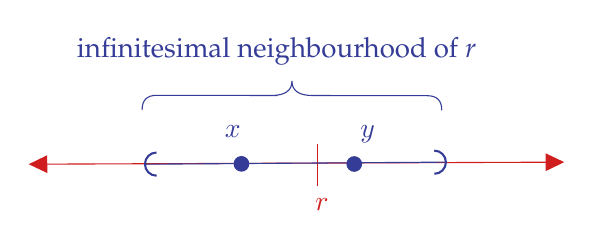
\begin{tikzpicture}[x=0.75pt,y=0.75pt,yscale=-1,xscale=1]
%uncomment if require: \path (0,119.19999694824219); %set diagram left start at 0, and has height of 119.19999694824219

%Straight Lines [id:da9254565786770808] 
\draw [color={rgb, 255:red, 208; green, 30; blue, 30 }  ,draw opacity=1 ]   (203.67,74.59) -- (457.67,73.61) ;
\draw [shift={(459.67,73.6)}, rotate = 539.78] [fill={rgb, 255:red, 208; green, 30; blue, 30 }  ,fill opacity=1 ][line width=0.75]  [draw opacity=0] (8.93,-4.29) -- (0,0) -- (8.93,4.29) -- cycle    ;
\draw [shift={(201.67,74.6)}, rotate = 359.78] [fill={rgb, 255:red, 208; green, 30; blue, 30 }  ,fill opacity=1 ][line width=0.75]  [draw opacity=0] (8.93,-4.29) -- (0,0) -- (8.93,4.29) -- cycle    ;
%Shape: Circle [id:dp5363573248589271] 
\draw  [color={rgb, 255:red, 53; green, 60; blue, 151 }  ,draw opacity=1 ][fill={rgb, 255:red, 53; green, 60; blue, 151 }  ,fill opacity=1 ] (300.65,74.43) .. controls (300.65,72.5) and (302.22,70.93) .. (304.15,70.93) .. controls (306.08,70.93) and (307.65,72.5) .. (307.65,74.43) .. controls (307.65,76.36) and (306.08,77.93) .. (304.15,77.93) .. controls (302.22,77.93) and (300.65,76.36) .. (300.65,74.43) -- cycle ;
%Shape: Circle [id:dp776984815602433] 
\draw  [color={rgb, 255:red, 53; green, 60; blue, 151 }  ,draw opacity=1 ][fill={rgb, 255:red, 53; green, 60; blue, 151 }  ,fill opacity=1 ] (355,74.5) .. controls (355,72.57) and (356.57,71) .. (358.5,71) .. controls (360.43,71) and (362,72.57) .. (362,74.5) .. controls (362,76.43) and (360.43,78) .. (358.5,78) .. controls (356.57,78) and (355,76.43) .. (355,74.5) -- cycle ;
%Straight Lines [id:da5309895801423343] 
\draw [color={rgb, 255:red, 208; green, 30; blue, 30 }  ,draw opacity=1 ]   (341,65.06) -- (341,85.06) ;


%Shape: Brace [id:dp4017562451998038] 
\draw  [color={rgb, 255:red, 53; green, 60; blue, 151 }  ,draw opacity=1 ] (400.67,48.6) .. controls (400.68,43.93) and (398.35,41.6) .. (393.68,41.59) -- (338.49,41.51) .. controls (331.82,41.5) and (328.49,39.17) .. (328.5,34.5) .. controls (328.49,39.17) and (325.16,41.5) .. (318.49,41.49)(321.49,41.49) -- (263.31,41.41) .. controls (258.64,41.4) and (256.31,43.73) .. (256.3,48.4) ;
%Straight Lines [id:da7018743824028313] 
\draw [color={rgb, 255:red, 53; green, 60; blue, 151 }  ,draw opacity=1 ]   (257.67,74.6) -- (402.67,73.6) ;
\draw [shift={(402.67,73.6)}, rotate = 539.6] [color={rgb, 255:red, 53; green, 60; blue, 151 }  ,draw opacity=1 ][line width=0.75]      (5.59,-5.59) .. controls (2.5,-5.59) and (0,-3.09) .. (0,0) .. controls (0,3.09) and (2.5,5.59) .. (5.59,5.59) ;
\draw [shift={(257.67,74.6)}, rotate = 359.6] [color={rgb, 255:red, 53; green, 60; blue, 151 }  ,draw opacity=1 ][line width=0.75]      (5.59,-5.59) .. controls (2.5,-5.59) and (0,-3.09) .. (0,0) .. controls (0,3.09) and (2.5,5.59) .. (5.59,5.59) ;

% Text Node
\draw (300,59.06) node [color={rgb, 255:red, 53; green, 60; blue, 151 }  ,opacity=1 ]  {$x$};
% Text Node
\draw (365,60.06) node [color={rgb, 255:red, 53; green, 60; blue, 151 }  ,opacity=1 ]  {$y$};
% Text Node
\draw (343,94.06) node [color={rgb, 255:red, 208; green, 30; blue, 30 }  ,opacity=1 ]  {$r$};
% Text Node
\draw (321,20) node [color={rgb, 255:red, 53; green, 60; blue, 151 }  ,opacity=1 ] [align=left] {infinitesimal neighbourhood of \textit{r}};


\end{tikzpicture}
\end{center}
\vspace{0.6em}
 }
 
%%%%%%%%%%%%%%%%%%%%%%%%%%%%%%%%%%%%%%%%%%%%%%%%%%%%%%%%%%%%%%%%%%%%%%%%%%%%%%
\headerbox{Lean Implementation}{name=lean,column=2,row=0}{
I formalised ultraproducts, the hyperreals and several important theorems about them in the formal proof-checker Lean -- my proofs were accepted in the Lean math library and most can be found in the following files at \cite{mathlib} under \texttt{/src/}:\vspace{-0.5em}
\begin{itemize}
    \item[--]\texttt{order/filter/filter\_product.lean} Ultraproduct, transfer properties (465 lines).\vspace{-0.5em}
    \item[--]\texttt{data/real/hyperreal.lean} -- hyperreals, their arithmetic (761 lines).
\end{itemize}
\vspace{-0.5em}
Some example theorems proved:\vspace{-0.5em}
\begin{itemize}
    \item[--] \texttt{instance [linear\_ordered\_field B] : linear\_ordered\_field B*}\vspace{-0.5em}
    \item[--] \texttt{st\_eq\_Sup \{x : R*\} : \\ st x = real.Sup \{y : R | y < x\}}\vspace{-0.5em}
    \item[--] \texttt{is\_st\_of\_tendsto \{f : N to R\} \{r : R\} (hf : tendsto f at\_top (nhds r)) :
  is\_st (of\_seq f) r}\vspace{-0.5em}
    \item[--] \texttt{def lift (f : B to B) : B* to B*} (proving it is well-defined)
\end{itemize}\vspace{-0.6em}
 }

%%%%%%%%%%%%%%%%%%%%%%%%%%%%%%%%%%%%%%%%%%%%%%%%%%%%%%%%%%%%%%%%%%%%%%%%%%%%%%
\headerbox{Non-standard analysis}{name=plots,column=1,span=2,below=comb}{
\textbf{Definition 1} -- For a constant $c\in\mathbb{R}$, function $f:\mathbb{R}^k\to\mathbb{R}$ and relation $P:\mathbb{R}^k\to\mathrm{Prop}$ we define their ``transfers'' $\hat{c}\triangleq[(c)]$, $\hat{f}([(r_i^1)],\ldots[(r_i^k)])\triangleq[(f(r_i^1,\ldots r_i^k))]$ and $\hat{P}([(r_i^1)],\ldots[(r_i^k)])\triangliff \{i \mid P(r_i^1,\ldots r_i^k)\}\in\phi$.\\
(exercise: prove this is well-defined -- note that $[(a_i)]$ is the hyperreal generated by the sequence $(a_i)$.)

\smallskip

\textbf{\Los's Theorem} (model theory) -- Extending $\mathbb{R}$-language to $\hat{\mathbb{R}}$ with Definition 1 -- for a formula $\pi$, we have: $\hat{\mathbb{R}}\models\pi([(x_i^1)],\ldots [(x_i^k)])\iff\{i \mid \mathbb{R}\models\pi(x_i^1,\ldots x_i^k)\}\in\phi$. In particular if $\pi$ is a sentence, $\mathbb{R}\models\pi\iff\hat{\mathbb{R}}\models\pi$.

\vspace{0.3em}

\emph{Proof:} Noting that the theorem is definitionally true for atomic formulae, we proceed by induction on formulae. Given the theorem for two formulae $\psi$, $\psi'$, we must show its validity for: 

\begin{enumerate}\vspace{-0.7em}
\item $\pi=\lnot\psi$: \ $\hat{\mathbb{R}}\models\lnot\psi \iff \{i\mid\mathbb{R}\models\psi\}\notin\phi \iff \{i\mid\mathbb{R}\models\lnot\psi\}\in\phi$. 
\vspace{-0.7em}
\item $\pi=\psi\land\psi'$: \ $\hat{\mathbb{R}}\models\psi\land\psi' \iff \{i\mid\mathbb{R}\models\psi\}\in\phi\land \{i\mid\mathbb{R}\models\psi'\}\in\phi \iff \{i\mid\mathbb{R}\models\psi\land\psi'\}\in\phi$. 
\vspace{-0.7em}
\item $\pi=\exists x, \psi(x)$: \ $\hat{\mathbb{R}}\models\exists x, \psi(x) \iff \exists x, \{i\mid\mathbb{R}\models\psi(x_i)\}\in\phi \iff \{i\mid \mathbb{R}\models\exists x_i,\psi(x_i)\}$. 
\end{enumerate}\vspace{-0.8em}

\smallskip

\textbf{Definition 2} -- A function $f : {\mathbb{R}}\to {\mathbb{R}}$ is said to (where $E$ is the set of infinitesimals) have \emph{limit} $L\in\mathbb{R}$ at $c$ if $\forall h\in E/\{0\},\ \st(\hat{f}(c+h))=L$. The definitions of derivatives and continuity follow in the standard way.

\smallskip

\textbf{Theorem 1} (connection to real analysis) -- Definition 2 is equivalent to the standard definition of a limit.

\vspace{0.3em}

\emph{Proof:} The backward implication is obvious. For the pullback: $\forall h \in E/\{0\}, f(c + h) - L \in E$ implies (with $\varepsilon$ real) $\forall \varepsilon>0,\forall h \in E', |f(c + h)-L|<\varepsilon \Rightarrow \forall\varepsilon>0, \exists \delta > 0, \forall h \in (0,\delta),  |f(c + h)-L|<\varepsilon $. Although $\varepsilon$ here is real, we may still transfer the remaining formula to the reals -- so $\{i\mid \exists\delta>0,\forall h\in(0,\delta),|f(c+h)-L|<\varepsilon_i\}\in\phi$. But since $\varepsilon$ is real, $\varepsilon_i$ can be a constant sequence, and the set must be the universe.

\medskip

The same principles as above may be used to formalise integrals, limits of sequences and other things from analysis. The above proof can also be almost identically repeated for the ultraproduct of a general Banach space -- in this case the non-standard derivative becomes equivalent to the Fr\'echet derivative. Formalisation of model theory and first-order logic in Lean is still complicated, thus non-standard analysis remains to be formalised in Lean. 

  \vspace{0.3em}
  }

%%%%%%%%%%%%%%%%%%%%%%%%%%%%%%%%%%%%%%%%%%%%%%%%%%%%%%%%%%%%%%%%%%%%%%%%%%%%%%
  \headerbox{More analysis}{name=discrete,column=3,row=0}{
(appendix of non-standard definitions, proofs)

\smallskip

\textbf{Definition 3} -- A sequence $a : \mathbb{N}\to\mathbb{R}$ has \emph{limit} $L$ if $\forall N\in\hat{\mathbb{N}}/\mathbb{N},\ \st(\hat{a}_N)=L$. Proof analogous to Thm 1.

\textbf{Definition 4} -- The sum $\hat{F}(N)=\hat{\sum}_{n=0}^N f(n)$ is the transfer of the partial-sum $F(K)=\sum_{k=0}^K f(k)$. Equivalence of convergent case analogous to Def 3.

Ex: $\int_{0}^xx^2dx=\st\sum_0^{\frac{x}{\varepsilon}}(k\varepsilon^2)\ \varepsilon=\st\left(\frac{x^3}3+\frac{x^2}2\varepsilon+\frac{x^2}6\varepsilon^2\right)$

\smallskip

\textbf{Theorem 2} (extreme value) -- Infinitesimally partition the interval. The mesh is hyperfinite, so by transfer, $\hat{f}$ has a maximum at $x_0$. By continuity, $\st(x_0)$ is the max of $f$. Analogously prove IVT, MVT.

\smallskip

\textbf{Definition 5} (non-standard Banach) -- standard part, limit defined as before; ``simultaneous transfer'' useful to define a hyperreal magnitude, and for analysis of functions $f:U\to V$. So it's straightforward to see, as in Thm 1, that the following definition is equivalent to the Fr\'echet derivative:
\vspace{-0.6em}
$$\forall h \in E_U/\{0\}, \frac{\|f(x+h)-f(x)-f'(x)h\|_V}{\|h\|_U}\in E_R$$
\vspace{-1.2em}
 \vspace{0.3em}
  }

%%%%%%%%%%%%%%%%%%%%%%%%%%%%%%%%%%%%%%%%%%%%%%%%%%%%%%%%%%%%%%%%%%%%%%%%%%%%%%
\headerbox{Conclusions}{name=concl,column=3,below=discrete}{
We have defined and investigated ultraproducts and hyperreal arithmetic with the aim of formalising infinitesimals and non-standard analysis. We have stated and proven several theorems about analysis in the non-standard setting, and proven the ``transfer principle'' to/from standard analysis. 

\smallskip

While I have formalised filters, ultraproducts and hyperreal algebra in Lean, non-standard analysis remains to be formalised -- well, that's easy, but the transfer principle will require formalising model theory and first-order logic in Lean. The Bernstein-Robinson theorem may also be worth formalising.

 }
  
%%%%%%%%%%%%%%%%%%%%%%%%%%%%%%%%%%%%%%%%%%%%%%%%%%%%%%%%%%%%%%%%%%%%%%%%%%%%%%
  \headerbox{References}{name=references,column=3,below=concl}{
    \smaller
    \vspace{-0.4em}
    \bibliographystyle{plain}
    \renewcommand{\section}[2]{\vskip 0.05em}
      \begin{thebibliography}{1}\itemsep=-0.01em
      \setlength{\baselineskip}{0.4em}
      \bibitem{mathlib}
        Lean Prover Mathematics Library.\\ \url{github.com/leanprover/mathlib}: Microsoft Research; 2019.
      \bibitem{hypr}
        Fabrizio G. 
        The Way of the Infinitesimal [Internet]. 2017 [cited 6 June 2019]. Available from: \url{https://arxiv.org/abs/1707.00459}.
    \bibitem{lang}
        Lang S. 
        Algebra (Graduate Texts on Mathematics: 211). 3rd ed. 
        New York: Springer-Verlag; 2002.
      \bibitem{arx}
        Cowles J, Gamboa R. 
        Equivalence of the Traditional and Non-Standard Definitions of Concepts from Real Analysis. 
        EPTCS. 2014; 152: 89-100.
      \bibitem{marker}
        Marker D.
        Model Theory: An Introduction (Graduate Texts on Mathematics: 217). 
        New York: Springer-Verlag; 2002.      \end{thebibliography}
  }

%%%%%%%%%%%%%%%%%%%%%%%%%%%%%%%%%%%%%%%%%%%%%%%%%%%%%%%%%%%%%%%%%%%%%%%%%%%%%%
  
\end{poster}

\end{document}
